\section{Use Cases}

In the past three years since the introduction of declarative
networking and the release of the \Pitu~\cite{p2} and DSN~\cite{dsn}
declarative networking systems, several applications have been
developed. We describe two of the original use cases that motivated
our work and drove several of our language and system designs: {\em
  safe extensible routers} and {\em overlay network development}.

%~\cite{mobiarch}, ~\cite{meld}.~\cite{Belaramani2009}, ~\cite{shenker}, 
%~\cite{SinghNSDI08}, ~\cite{declarativeSensors,chu07,chu09},
%~\cite{mosaicConext},~\cite{presto08}, 

\subsection{Declarative Routing}

The Internet's core routing infrastructure, while arguably robust and
efficient, has proven to be difficult to evolve to accommodate the
needs of new applications. Prior research on this problem has included
new hard-coded routing protocols on the one hand, and fully extensible
Active Networks on the other. {\em Declarative
  routing}~\cite{declareRoute} explores a new point in this design
space that aims to strike a better balance between the extensibility
and robustness of a routing infrastructure.

With declarative routing, a routing protocol is implemented by writing
a simple query in \Dlog, which is then executed in a distributed
fashion at some or all of the nodes. Declarative routing can be viewed
as a restrictive instantiation of Active Networks for the control
plane, which aims to balance the concerns of expressiveness,
performance and security, properties which are needed for an
extensible routing infrastructure to succeed.

Security is a key concern with any extensible system particularly when
it relates to the consumption of resources due to extensions.  \Dlog
is amenable to static analysis due to its connections to Datalog. {\em
  Pure} Datalog (without any negation, aggregation or function symbols) has
polynomial time and space complexities in the size of the
input~\cite{alicebook}. This property provides a natural bound on the
resource consumption. However, many extensions of Datalog (including
\Dlog) augment the core language in various ways,
extending its polynomial complexity.

Fortunately, static analysis tests have been developed to check for
the termination of an augmented Datalog query on a given
input~\cite{krs}. In a nutshell, these tests identify recursive
definitions in the query rules, and check whether these definitions
terminate. Examples of recursive definitions that terminate are ones
that evaluate monotonically increasing (decreasing) predicates whose
values are upper (lower) bounded. Moreover, the declarative framework is
amenable to other verification techniques, ranging from theorem
proving~\cite{dnv}, model checking~\cite{card}, and runtime
verification~\cite{singhEurosys}.



%Runtime verification~\cite{singhEurosys} is a mechanism for checking
%at runtime that a system does not violate expected properties.  Since
%declarative networks utilize a distributed query engine to execute its
%protocols, these checks can be expressed as {\em monitoring
%  queries}~\cite{singhEurosys} in \Dlog.  Examples include queries for
%monitoring for inconsistent routing or structural property violations
%of networks.


%\reminder{Safety. Talk about model checking~\cite{card}, mechanized theorem
%provers~\cite{dnv}, synthesizing verified specifications~\cite{tpdn},
%etc.}

\Dlog can express a variety of well-known routing protocols (e.g.,
distance vector, path vector, dynamic source routing, link state,
multicast) in a compact and clean fashion, typically in a handful of
lines of program code. Moreover, higher-level routing concepts (e.g.,
QoS constraints) can be achieved via simple modifications to these
queries. Finally, writing the queries in \Dlog illustrates surprising
relationships between protocols.  For example, we have shown that
distance vector and dynamic source routing~\cite{dsr} differ only in a
simple, traditional query optimization decision: the order in which a
query's predicates are evaluated.

To limit query computation to the relevant portion of the network, we
use a query rewrite technique, called {\em magic sets
  rewriting}~\cite{oldMagic}. Rather than reviewing the Magic Sets
optimization here, we illustrate its use in an example: by modifying
rules \nd{sp1-sp4} from the path-vector program, the following computes only
paths limited to sources/destinations in the
\nd{magicSrc}/\nd{magicDst} tables respectively.

\begin{NDlog}
sp1-sd pathDst(@D,S,D,P,C) :- magicSrc(@S), link(@S,D,C),
          P = f\_concatPath(link(@S,D,C), nil). 
sp2-sd pathDst(@D,@S,@Z,P,C) :- pathDst(@Z,@S,Z1,P1,C1),
          link(@Z,@D,C2), C := C1 + C2, 
          P = f\_concatPath(P1,link(@Z,D,C2)).
sp3-sd spCost(@D,S,min<C>) :- magicDst(@D), pathDst(@D,S,Z,P,C).
sp4-sd shortestPath(@D,S,P,C) :- spCost(@D,S,C),
           pathDst(@D,S,Z,P,C).
\end{NDlog}

Our evaluation results~\cite{declareRoute} based on running
declarative routing protocols on PlanetLab and in a local cluster show
that when all nodes issue the same query, the query execution has
similar scalability properties as the traditional distance vector and
path vector protocols. For example, the convergence latency for the
path-vector program is proportional to the network diameter, and
converges in the same time compared to the path vector
protocol. Second, the per-node communication overhead increases
linearly with the number of nodes. This suggests that our approach
does not introduce any fundamental overheads. Moreover, when there are
few nodes issuing the same query, query optimization and work-sharing
techniques can significantly reduced the communication overhead.

One promising direction stems from our surprising observation on the
synergies between query optimization and network routing: a wired
protocol such as the distance-vector protocol can be translated to a
wireless protocol by applying the standard database optimizations of
magic sets rewrite and predicate reordering.  More complex applications of 
query optimization have begun to pay dividends in research research, synthesizing new hybrid protocols from traditional building blocks~\cite{chu09,chuthesis}
Given the proliferation
of new routing protocols and a diversity of new network architecture
proposals, the connection between query optimizations and network
routing suggests that query optimizations may help us inform new
routing protocol designs and allow the hybridization of protocols
within the network.

%due to a wide range of
%variability in network connectivity and also a wide range of data
%traffic patterns, a {\it one-size-fits-all} routing algorithm does not
%exist.  







%\jmh{We need to highlight the biggest nugget here: flexibility between DVR and DSR, the ``upleveling'' of protocol design to query optimization.}





\subsection{Declarative Overlays}
%\petros{Get rid of this, doesn't add much.}
%\reminder{To be fixed}

In declarative routing, we demonstrated the flexibility and
compactness of \Dlog for specifying a variety of routing protocols.
In practice, most distributed systems are much more complex than
simple routing protocols; in addition to routing, they typically also
perform application-level message forwarding and handle the formation
and maintenance of a network as well.

\eat{ All large-scale distributed systems inherently use one or more
  application-level overlay networks as part of their operation.  In
  some cases, the overlay is prominent: for example, file-sharing
  networks maintain neighbor tables to route queries.  In other
  systems, the overlay or overlays may not be as explicit: for
  example, Microsoft Exchange email servers within an enterprise
  maintain an overlay network among themselves using a link-state
  algorithm over TCP for routing mail and status messages.}

In our subsequent work on {\em declarative
  overlays}~\cite{declareOverlays}, we demonstrate the use of \Dlog to
implement practical application-level overlay networks. In declarative
overlays, applications submit to \Sys a concise \Dlog program which
describes an overlay network, and the \Sys system executes the program
to maintain routing tables, perform neighbor discovery and provide
forwarding for the overlay.

\eat{A typical overlay network consists of three functionalities: 

\begin{itemize}
\item {\bf Routing} involves the computation and maintenance of routing
  tables at each node based on input neighbor tables. This functionality
  is typically known as the {\em control plane} of a network.
\item {\bf Forwarding} involves the delivery of overlay messages along
  the computed routes based on the destination addresses of the
  messages. This functionality is typically known as the {\em
  forwarding} plane of a network.
\item {\bf Overlay formation and maintenance} involves the process of
  joining an overlay network and maintaining the neighbor set at each
  node. The selected neighbors are used as input to the control plane
  for route computations.
\end{itemize}}

In declarative routing, \Dlog programs are used solely for programming
the control plane. Hence, all routing examples consist of \Dlog rules
that compute routes based on input links. On the other hand, in
declarative overlays, the \Sys system resides at the application
level, and all messages are routed via the default Internet
routing. Here, \Dlog programs implement the additional functionalities
of neighbor discovery, maintenance, and message forwarding. 

These programs are more complex due to the handling of message
delivery, acknowledgments, failure detection and timeouts required by
the additional functionalities. The programs also heavily utilize
soft-state data and soft-state rules.  Despite the increased
complexity, we demonstrate that our \Dlog programs are significantly
more compact compared to equivalent C++ implementations. For instance,
the use of \Dlog for expressing two complex overlay networks, namely
the Narada mesh formation and a full-fledged implementation of the
Chord distributed hash table in \PNaradaLines and \PChordLines rules
respectively. 

In the case of the Chord DHT, there are rules for performing various
aspects of Chord, including initial joining of the Chord network,
Chord ring maintenance, finger table maintenance, recursive Chord
lookups, and failure detection of neighbors. The detailed Chord
specifications are available in \cite{boonThesis}.

We note that our Chord implementation is roughly two orders of
magnitude less code than the original C++ implementation. This is a
quantitative difference that is sufficiently large that it becomes
qualitative: in our opinion (and experience), declarative programs
that are a few dozen lines of code are markedly easier to understand,
debug and extend than multi-thousand-line imperative programs.
Moreover, we demonstrate in ~\cite{boonThesis,declareOverlays} that
our declarative overlays achieve the expected high-level properties of
their respective overlay networks for both static and dynamic
networks. For example, in a static network of up to $500$ nodes, the
measured hop-count of lookup requests in the Chord network conformed
to the theoretical average of $0.5 \times log_{2}N$ hops, and the
latency numbers were within the same order of magnitude as published
Chord numbers.



 





\eat{
\reminder{Describe Chord in 41 lines briefly. How many rules for doing
  what. Show the recursive lookup rules. }

\reminder{Show the lookup rules of Chord}

In this section, we focus on measuring the full Chord DHT specification
in Appendix~\ref{sec:appendixExamples:chordOverlog}. Chord is a good
stress test of our architecture, being relatively complex compared to
other overlay examples like gossip and end-system multicast.  Chord also
has the advantage of being well-studied. Our \Sys-Chord deployment on
the Emulab testbed~\cite{emulab} consists of $100$ machines executing up
to $500$ \Sys-Chord instances ($5$ \Sys processes running on each Emulab
machine). We utilize the same network topology as the Narada
experiment. Since we are running up to $5$ \Sys processes per Emulab
node, we selected Emulab machines with newer hardware (64-bit Xeon 3000
series with $2$ GB memory) to run our experiments.

\begin{figure*}[ht]
\centering
 \begin{minipage}{.3\linewidth}
  \begin{center}
    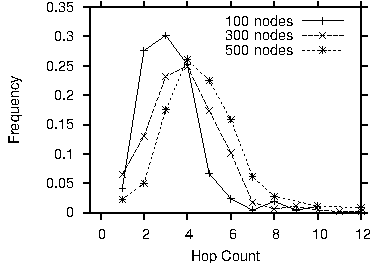
\includegraphics[width=2in]{graphs/overlays/hop_lookup.pdf}
    \caption{{\small Hop-count distribution for lookups.}\label{chord-hop}}
 \end{center}
%\end{figure}
\end{minipage}
\hfill
 \begin{minipage}{.3\linewidth}
%\begin{figure}[ht]
  \begin{center}
    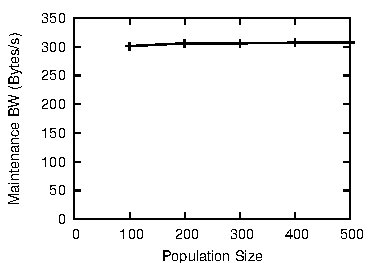
\includegraphics[width=2in]{graphs/overlays/noChurnBW.pdf}
    \caption{{\small Maintenance traffic for different network sizes.}\label{chord-bw}}
  \end{center}
%\end{figure}
 \end{minipage}
\hfill
 \begin{minipage}{.3\linewidth}
%\begin{figure}[ht]
  \begin{center}
    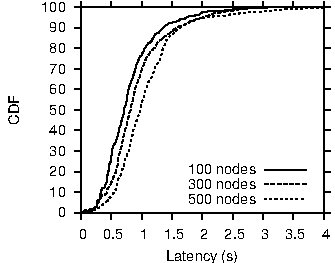
\includegraphics[width=2in]{graphs/overlays/noChurnLatencyCDF.pdf}
    \caption{{\small CDF for lookup latency.}\label{chord-latency}}
  \end{center}
 \end{minipage}
\end{figure*}

%OP\subsubsection{Static Network Validation}

In our first round of experiments, we validate the high-level
characteristics of the Chord overlay. We generate a uniform workload
of DHT ``lookup'' requests to a static set of nodes in the overlay,
with no nodes joining or leaving.  This is somewhat unrealistic but it
allows us to ensure we are achieving the static properties of
Chord. In each experiment, we start a landmark node, and have all
other nodes join the landmark node at regular intervals. Once all the
nodes have joined the Chord overlay, we issue lookups every $15$
seconds simultaneously (with the same lookup key $K$) from $10$ nodes.

Figure~\ref{chord-hop} shows the hop-count distribution for our
workload.  Except for a few outliers, $99\%$ of all lookups complete
within $10$ hops. The average hop count of lookups are $3.3$, $4.0$ and
$4.5$ for node sizes of $100$, $300$ and $500$ respectively,
approximating the theoretical average of $0.5 \times log_{2}(N)$, where $N$ is
the number of nodes.  

Figure~\ref{chord-latency} shows the CDF of lookup latencies for
different network sizes.  As expected, the average latency increases in
proportion to the average lookup hop count for each network size. On a
$500$ node static network, $99\%$ of all lookups complete in less than
$3.4$ seconds. The average (median) latencies are $0.81$ seconds ($0.72$
seconds), $0.92$ seconds ($0.82$ seconds) and $1.09$ seconds ($0.98$
seconds) for node sizes of $100$, $300$ and $500$ respectively. Our
average and median latency numbers are within the same order of
magnitude as the published numbers~\cite{chord} of the MIT Chord
deployment. 

In addition to achieving expected latency numbers, our lookups are also
``correct''. All lookup requests return successfully with the lookup
requests. In addition, all lookups achieve $100\%$ consistency, where
all lookup requests for the same key issued from different nodes return
identical results.

\begin{figure}[ht]
  \begin{center}
    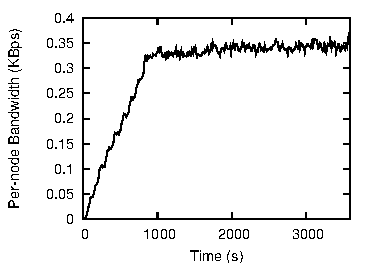
\includegraphics[width=3in]{graphs/overlays/bw.pdf}
    \caption{{\small Per-node Bandwidth (KBps) over time (s).}\label{chord-bw}}
  \end{center}
% \end{minipage}
\end{figure}


Figure~\ref{chord-bw} shows the per-node bandwidth (KBps) consumption
over time (in seconds) for a static \Sys-Chord network where fingers are
fixed every $10$ seconds, and ring stabilization (exchange of successors
and predecessors among neighbors) happen every $10$ seconds. Each node
periodically send ping messages to neighbors every $3$ seconds. After an
initial linear increase in bandwidth as nodes join the Chord ring, the
bandwidth utilization stabilizes at $0.34$ KBps, well within the
published bandwidth consumption of $1$ KBps~\cite{bamboo} of other high
consistency and low latency DHTs.
}



%\subsection{Other Use Cases}

